\documentclass[oneside, 11pt]{article}

\usepackage[T1]{fontenc}
\usepackage[utf8]{inputenc}
\usepackage[english]{babel}

\usepackage{fouriernc}
\usepackage[detect-all, binary-units, separate-uncertainty=true,
            per-mode=symbol, retain-explicit-plus, retain-unity-mantissa=false]{siunitx}

\usepackage{setspace}
\setstretch{1.2}

\setlength{\parskip}{\smallskipamount}
\setlength{\parindent}{0pt}

\usepackage[headheight=14pt]{geometry}
\geometry{marginparwidth=0.5cm, verbose, a4paper, tmargin=3cm, bmargin=3cm,
          lmargin=2cm, rmargin=2cm}

\usepackage{float}

\usepackage[fleqn]{amsmath}
\numberwithin{equation}{section}
\numberwithin{figure}{section}

\usepackage{graphicx}
\graphicspath{{images/}{../../../images/}}

\usepackage{tikz}
\usetikzlibrary{shapes}
\usetikzlibrary{plotmarks}

\newcounter{Exercise}
\setcounter{Exercise}{1}
\usepackage{xcolor}
\definecolor{shadecolor}{gray}{0.9}
\usepackage{framed}
\usepackage{caption}

\usepackage{url}


\usepackage{fancyhdr}
\pagestyle{fancy}
\fancyhf{}
\rhead{\thepage}
\renewcommand{\footrulewidth}{0pt}
\renewcommand{\headrulewidth}{0pt}

\fancypagestyle{firststyle}
{
    \fancyhf{}
    \rhead{\thepage}
    \cfoot{
\includegraphics[height=30pt]{HiSPARClogo}}
    \rfoot{
\includegraphics[height=25pt]{CCbysa}}
    \lfoot{
\includegraphics[height=30pt]{NIKHEFlogo}}
    \renewcommand{\footskip}{50pt}
    \renewcommand{\footrulewidth}{0.1pt}
    \renewcommand{\headrulewidth}{0pt}
}

\newcommand{\figref}[1]{Figuur~\ref{#1}}

\newcommand{\hisparc}{\textsmaller{HiSPARC}\xspace}
\newcommand{\kascade}{\textsmaller{KASCADE}\xspace}
\newcommand{\sapphire}{\textsmaller{SAPPHiRE}\xspace}
\newcommand{\jsparc}{\textsmaller{jSparc}\xspace}
\newcommand{\hdf}{\textsmaller{HDF5}\xspace}
\newcommand{\aires}{\textsmaller{AIRES}\xspace}
\newcommand{\csv}{\textsmaller{CSV}\xspace}
\newcommand{\python}{\textsmaller{PYTHON}\xspace}
\newcommand{\corsika}{\textsmaller{CORSIKA}\xspace}
\newcommand{\labview}{\textsmaller{LabVIEW}\xspace}
\newcommand{\daq}{\textsmaller{DAQ}\xspace}
\newcommand{\adc}{\textsmaller{ADC}\xspace}
\newcommand{\hi}{\textsc{h i}\xspace}
\newcommand{\hii}{\textsc{h ii}\xspace}
\newcommand{\mip}{\textsmaller{MIP}\xspace}
\newcommand{\hisparcii}{\textsmaller{HiSPARC II}\xspace}
\newcommand{\hisparciii}{\textsmaller{HiSPARC III}\xspace}

\DeclareSIUnit{\electronvolt}{\ensuremath{\mathrm{e\!\!\:V}}}

\DeclareSIUnit{\unitsigma}{\ensuremath{\sigma}}
\DeclareSIUnit{\mip}{\textsmaller{MIP}}
\DeclareSIUnit{\adc}{\textsmaller{ADC}}

\DeclareSIUnit{\gauss}{G}
\DeclareSIUnit{\parsec}{pc}
\DeclareSIUnit{\year}{yr}



\begin{document}

\title{Detecteren}
\author{N.G. Schultheiss}
\date{}

\maketitle
\thispagestyle{firststyle}

\section{Inleiding}

De HiSPARC-detector neemt kosmische deeltjes waar. De detector bestaat
uit een scintilatorplaat van 0,50m bij 1,00m waaraan een lichtgeleider
is gelijmd. Een deel van het licht wordt hiermee naar een lichtdetector
geleid. In deze module kijken we naar de lichtgeleidende eigenschappen
van de scintillator. In de hier op volgende module ``Scintillatie''
wordt het scintillatiemechanisme verder bekeken. 


\section{De constructie van de detector}

De HiSPARC-detector neemt kosmische deeltjes waar. Dit gebeurt doordat
het deeltje op een scintillatorplaat van 0,50{[}m{]} bij 1,00{[}m{]}
valt. Het deeltje veroorzaakt in de scintillatorplaat een aantal fotonen
met een golflengte van 425nm. Deze fotonen worden ten dele via een
lichtgeleider naar de photomultiplier (lichtdetector) geleid.

\begin{figure}[H]
\noindent \begin{centering}
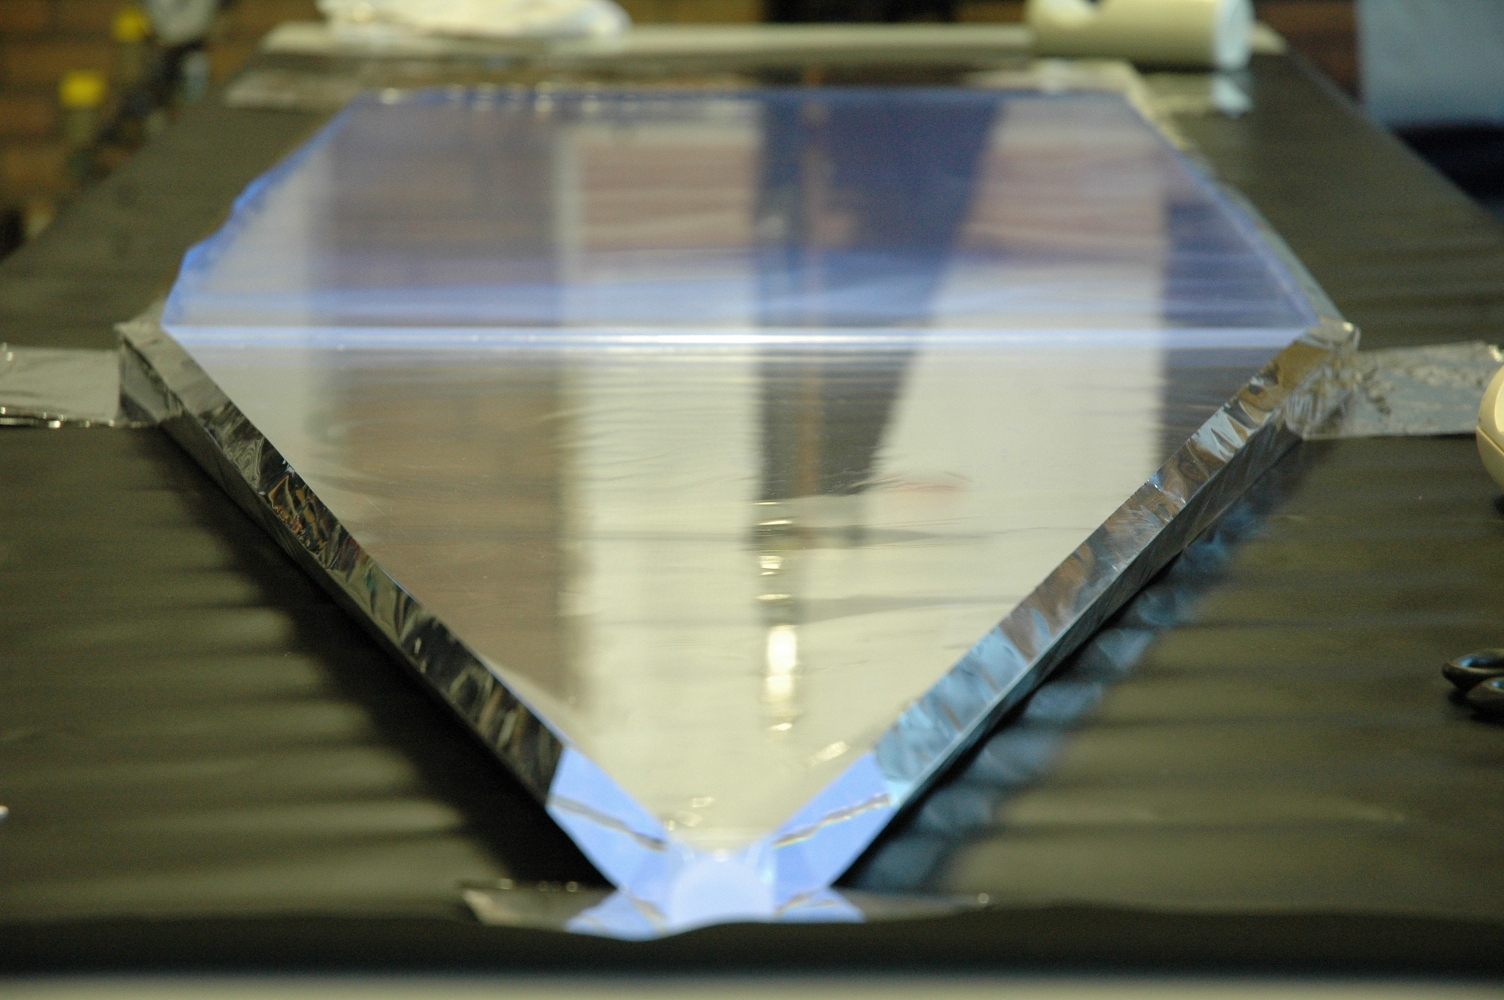
\includegraphics[width=15cm]{DSC_0081}
\par\end{centering}
\caption{De scintilatorplaat met de lichtgeleider}
\end{figure}


De fotonen in de scintilatorplaat ontstaan door fluorescentie. Bij
fluorescentie wordt een deel van de energie van een invallend deeltje
gebruikt om een atoom in een aangeslagen \footnote{Als een atoom in een
aangeslagen toestand komt, wordt een electron van de grondtoestand naar
een hoger energieniveau gebracht. Even later valt het electron weer
terug onder uitzending van een foton met deze gedefineerde energie.}
toestand te brengen. Even later valt het atoom terug in de
grondtoestand. De energie komt bij de terugval vrij als fluoriserende
straling.

Helaas kan gewoon licht, en ook UV-straling, de atomen in een aangeslagen
toestand brengen. Verder reageert de detector ook op ander licht dan
het fluorescentie licht. Het is dus noodzakelijk om de HiSPARC-detector
goed lichtdicht te verpakken. Een lichtlekje leidt direct tot een
serie valse metingen.

Het zou prettig zijn als de grootte van de lichtpuls alleen afhangt
van de energie van het deeltje en niet van de plaats waar het deeltje
op de detector valt. Als de lichtdetector direct op de scintillatorplaat
wordt aangesloten, spreekt het voor zich dat pulsen die vlakbij de
detector ontstaan een veel hoger signaal geven dan de pulsen die ver
van de detector ontstaan. Door een lichtgeleider tussen de scintillatorplaat
en de detector te plaatsen, kunnen we dit effect grotendeels voorkomen.


\section{Theoretische evaluatie van de detector}

We kunnen het detectorontwerp theoretisch beschouwen als een lichtgeleider
bestaande uit een scintillatorplaat en de perspex driehoek. Zolang
de hoek van inval groter is dan de grenshoek zal er totale reflectie
optreden. Zoals in figuur 3.1 te zien is, treedt een deel van het
licht uit de lichtgeleider omdat de fluorescentiefotonen (lichtstralen)
in alle richtingen bewegen. Waarschijnlijk wordt dit licht voor een
deel door de aluminiumfolie rond de detector teruggekaatst. Bij iedere
weerkaatsing treedt een beetje absorptie op en verdwijnt een deel
van de fotonen. We mogen dus aannemen dat de uittredende fotonen een
verwaarloosbare bijdrage leveren aan het gedetecteerde licht. Verder
is te zien dat dit verlies niet afhangt van de plaats van de fluorescentie.
Er gaat altijd eenzelfde hoeveelheid licht verloren.

\begin{figure}[h]
\noindent \begin{centering}
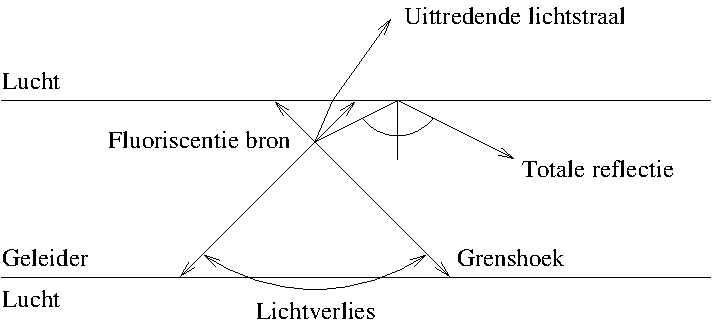
\includegraphics[scale=0.75]{lichtverlies}
\par\end{centering}

\caption{Lichtverlies in de lichtgeleider}
\end{figure}


We gaan uit van de gedachte dat het licht door de detector wordt geleidt.
In de module ``Het Heelal'' is te lezen dat de schijnbare helderheid
(intensiteit) omgekeerd kwadratisch evenredig is met de afstand. Het
is de vraag of we deze gedachte ook bij lichtgeleiders mogen gebruiken.


\paragraph*{Opdracht 1:}

\emph{In de module ``Het Heelal'' gaat het licht achtereenvolgens
door kubussen met oplopende grootte. Omdat het licht over het gehele
oppervlak wordt verdeeld, neemt de gemiddelde intensiteit kwadratisch
met de ribbe van de kubus af. In de lichtgeleider verspreidt het licht
dat niet verloren gaat zich min of meer in cilinders. Toon aan dat
de lichtintensiteit in een lichtgeleider omgekeerd evenredig is met
de afstand.}

\begin{figure}[H]
\noindent \begin{centering}
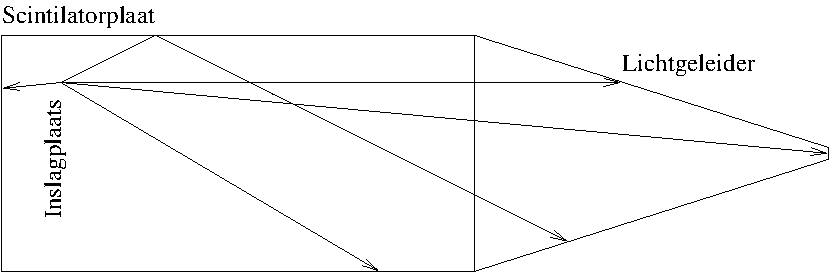
\includegraphics[scale=0.75]{bovenaanzicht}
\par\end{centering}

\caption{Bovenaanzicht van de detector}
\end{figure}


Het bovenaanzicht van de detector is in figuur 3.2 te zien. Op het
eerste gezicht lijkt het of de hoeveelheid licht bij de detector toeneemt,
doordat de geleider steeds smaller wordt. Zoals te zien is gaan we
uit van een kosmisch deeltje dat op de scintillatorplaat is ingeslagen.
Uiteraard gaan de lichtstralen alle kanten op. Eén lichtstraal gaat
direct naar de detector, dit licht wordt gemeten. Er zijn nog vier
andere stralen te zien.


\paragraph*{Opdracht 2:}

\emph{Maak de vier overgebleven stralen af en laat zien of deze stralen
in de detector kunnen komen. Leg hiermee uit of het smaller worden
van de lichtgeleider een grote verhoging van het gemeten signaal geeft.}

Op de wijze van figuur 3.2 is het niet eenvoudig om te onderzoeken
hoeveel stralen er in de detector komen. We gaan over op een nieuw
model waarin de lichtgeleider niet smaller wordt maar een rechthoek
is. Hierin zijn drie lichtstralen te zien die detector kunnen bereiken.
Het spreekt voor zich dat de spiegelbeelden ook weer spiegelbeelden
hebben.

\begin{figure}[H]
\noindent \begin{centering}
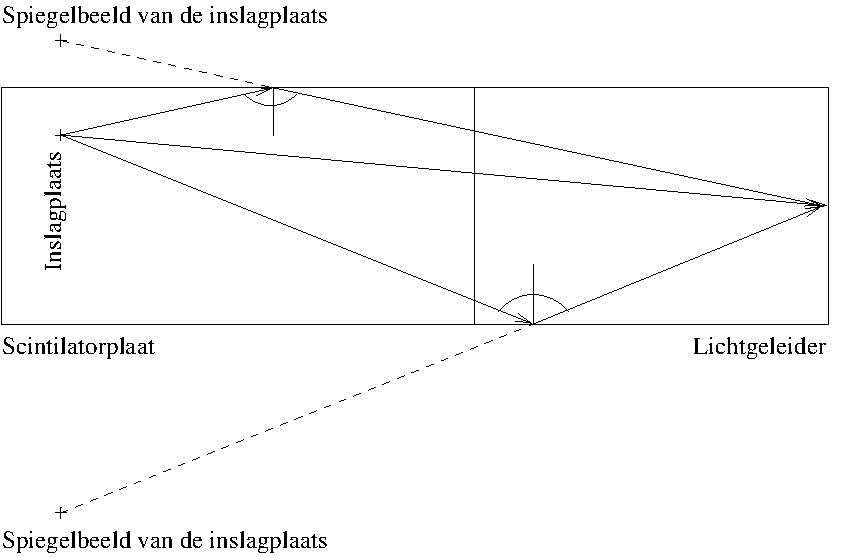
\includegraphics[scale=0.75]{bovenaanzicht1}
\par\end{centering}

\caption{Bovenaanzicht met spiegelbeelden}
\end{figure}


\paragraph*{Opdracht 3:}

\emph{Leg uit hoe de eisen voor de reflectie aan het oppervlak van
de detector het aantal mogelijke reflecties beperken.}


\paragraph*{Opdracht 4:}

\emph{Leg uit dat er meer lichtstralen bij de detector kunnen komen
als de afstand van het inslagpunt tot de detector toeneemt.}

Als model kunnen we uitgaan van twee gedachten:
\begin{itemize}
\item De intensiteit van de lichtbundel is omgekeerd evenredig met de afstand.
\item Het aantal mogelijke lichtbundels is rechtevenredig met de afstand.
\end{itemize}
Als deze kloppen dan is het signaal van de lichtdetector niet afhankelijk
van de plaats van inslag van de straling.


\paragraph*{Opdracht 5:}

\emph{Beargumenteer of het bovenstaande model te verdedigen is. }


\section{Een practische simulatie}

\begin{figure}[h]
\noindent \begin{centering}
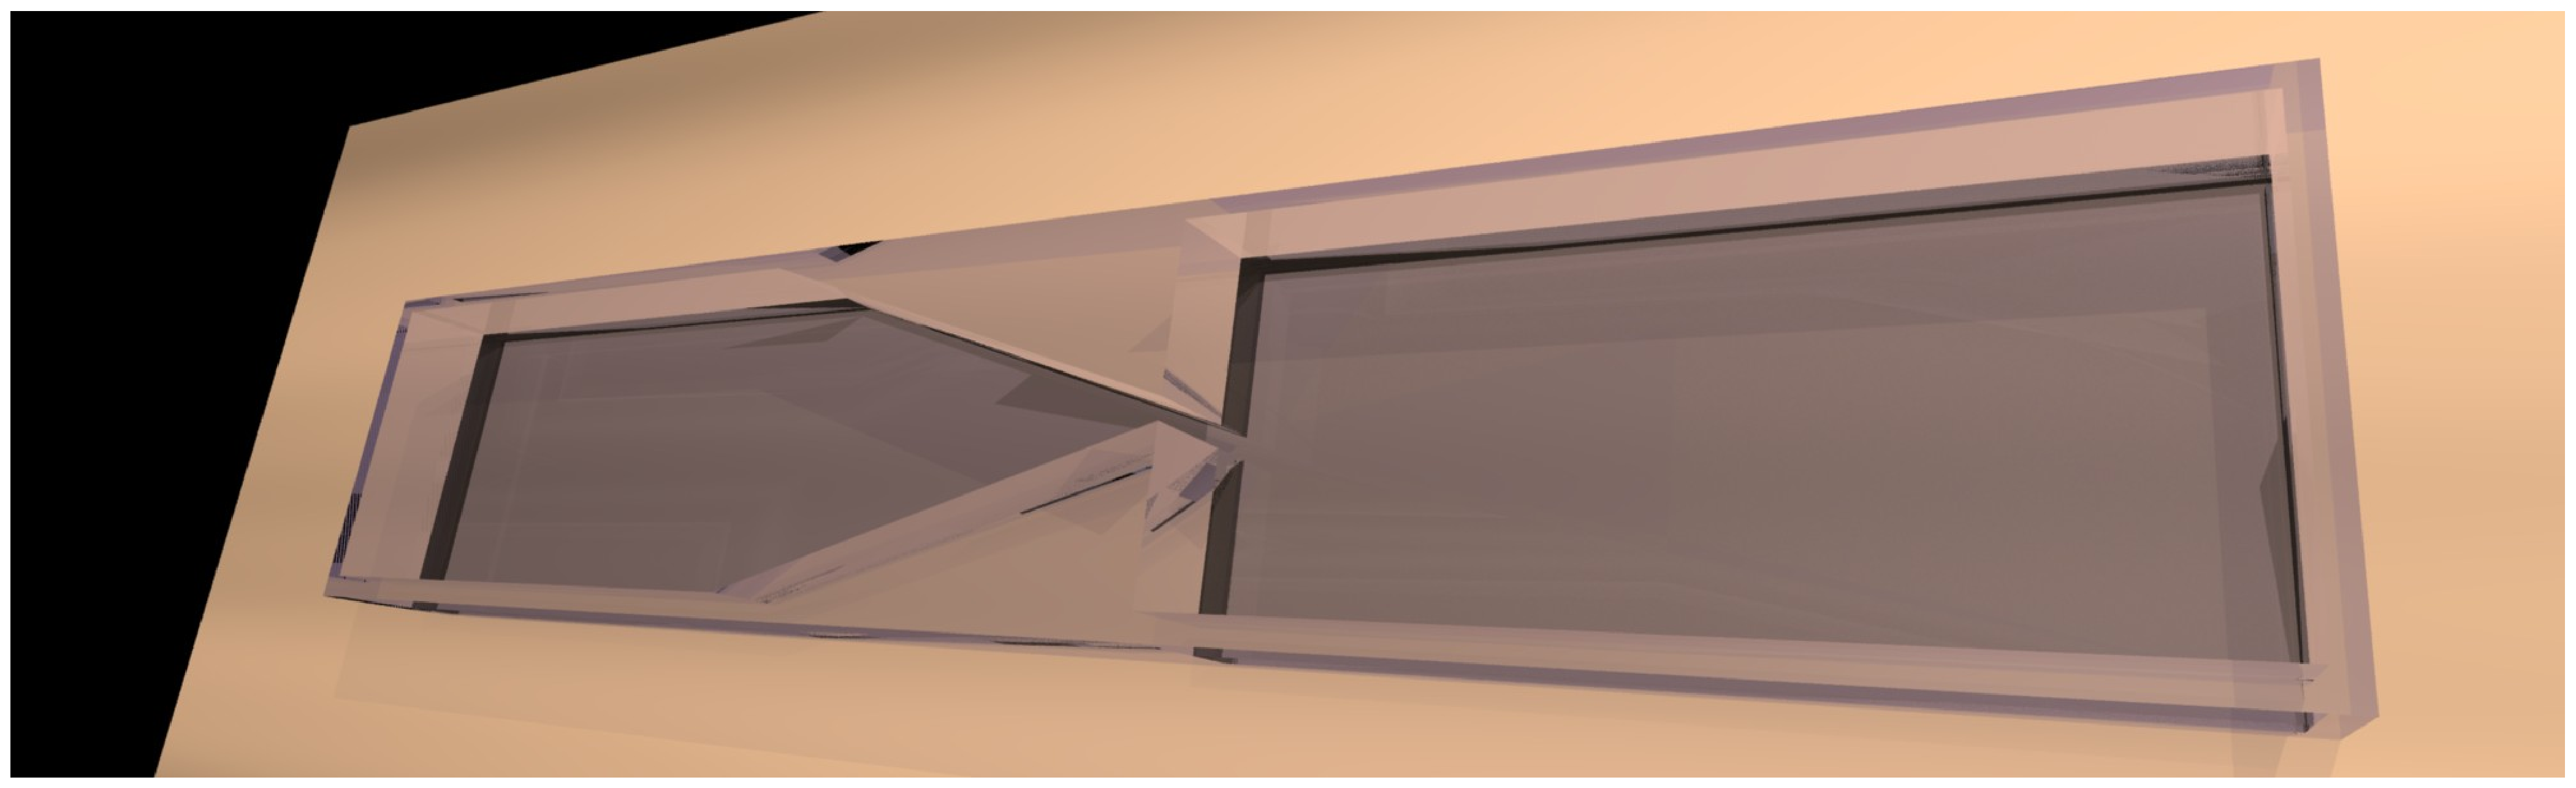
\includegraphics[width=15cm]{simulatie4}
\par\end{centering}

\caption{Een perspex simulatiebak}
\end{figure}


Deze theorie is te toetsen met een simulatie in een golfbak. Naast
de bak volgens figuur 4.1 is hiervoor nodig:
\begin{itemize}
\item Een druppelpipet.
\item Water.
\end{itemize}
We laten druppels water in de bak vallen. De energie van de druppel
wordt omgezet in een golf die zich over het wateroppervlak verspreidt.
De golf botst tegen de strook metaal en weerkaatst. Een deel van de
golf komt uit de opening bij de detector. De golf die ontsnapt is
te vergelijken met de hoeveelheid licht die in de lichtdetector valt.


\paragraph*{Opdracht 6:}

\emph{Als de hoek kleiner dan de grenshoek is, treedt er geen totale
reflectie meer op. Helaas houdt dit model geen rekening met deze
gedeeltelijke reflectie. Verzin hoe deze ``absorptie'' in het model kan
worden gerealiseerd.}

\end{document}
